\section{Additional memory results}
\label{app:memory}

\Cref{fig:weights,tab:weights} give the weight memory of every configuration and model size.
\Cref{fig:breakdown} splits the peak memory of the 7B model on HF into weights, KV cache and
activations. It shows why the run-time saving shrinks: as the batch grows, the KV cache and the
activations take a growing share of the peak memory, and neither is quantized. \Cref{fig:kvcap} shows the
KV-cache capacity that vLLM gets from the memory each format frees.

\begin{figure}[htbp]
\centering
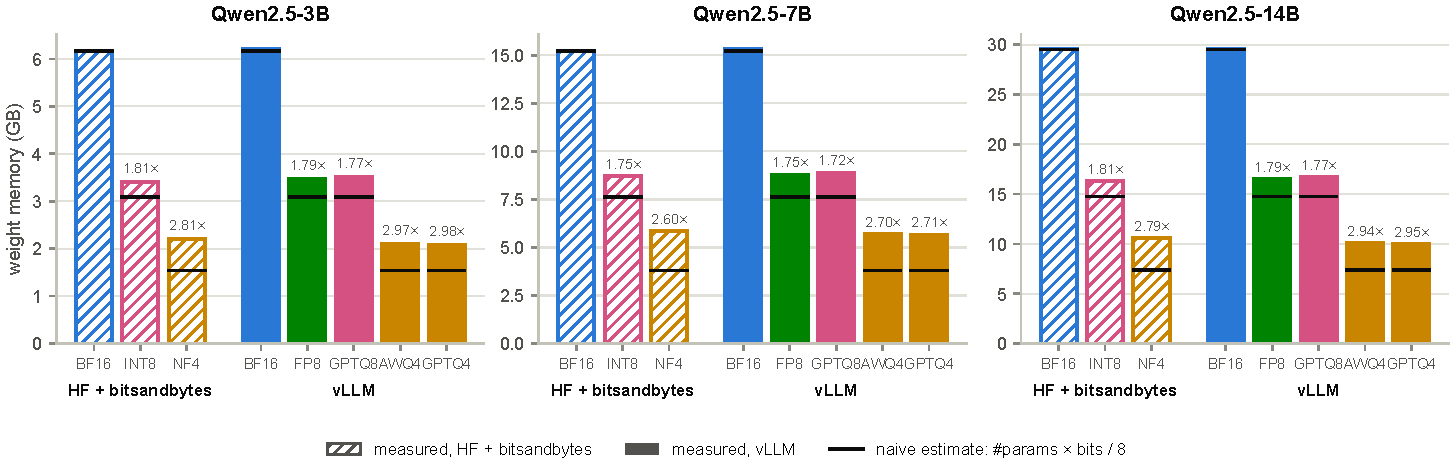
\includegraphics[width=\linewidth]{q1_weight_memory}
\caption{Weight memory of every configuration for the three Qwen2.5 sizes (bars: measured; black
ticks: $\#\text{params}\times\text{bits}/8$). Labels give the saving against BF16 on the same backend.}
\label{fig:weights}
\end{figure}

\begin{table*}[t]
\centering
\footnotesize
\caption{Q1 --- weight memory: naive estimate ($\#$params$\times$bits/8), our analytic model (unquantized embedding/LM head/norms + quantization metadata), and measured on the GPU.}
\label{tab:weights}
\setlength{\tabcolsep}{4pt}
\begin{tabular}{llrrrrr}
\toprule
Model & Config & Naive (GB) & Model (GB) & Measured (GB) & Ratio vs BF16 & Naive ratio \\
\midrule
Qwen2.5-7B & HF BF16 & 15.23 & 15.23 & 15.23 & 1.00$\times$ & 1.00$\times$ \\
Qwen2.5-7B & HF INT8 (LLM.int8) & 7.62 & 8.71 & 8.71 & 1.75$\times$ & 2.00$\times$ \\
Qwen2.5-7B & HF NF4 & 3.81 & 5.85 & 5.85 & 2.60$\times$ & 4.00$\times$ \\
Qwen2.5-7B & vLLM BF16 & 15.23 & 15.23 & 15.34 & 1.00$\times$ & 1.00$\times$ \\
Qwen2.5-7B & vLLM FP8 W8A8 & 7.62 & 8.71 & 8.77 & 1.75$\times$ & 2.00$\times$ \\
Qwen2.5-7B & vLLM GPTQ W8A16 & 7.62 & 8.86 & 8.90 & 1.72$\times$ & 2.00$\times$ \\
Qwen2.5-7B & vLLM AWQ W4A16 & 3.81 & 5.57 & 5.68 & 2.70$\times$ & 4.00$\times$ \\
Qwen2.5-7B & vLLM GPTQ W4A16 & 3.81 & 5.57 & 5.66 & 2.71$\times$ & 4.00$\times$ \\
Qwen2.5-14B & HF BF16 & 29.54 & 29.54 & 29.54 & 1.00$\times$ & 1.00$\times$ \\
Qwen2.5-14B & HF INT8 (LLM.int8) & 14.77 & 16.33 & 16.34 & 1.81$\times$ & 2.00$\times$ \\
Qwen2.5-14B & HF NF4 & 7.39 & 10.55 & 10.58 & 2.79$\times$ & 4.00$\times$ \\
Qwen2.5-14B & vLLM BF16 & 29.54 & 29.54 & 29.60 & 1.00$\times$ & 1.00$\times$ \\
Qwen2.5-14B & vLLM FP8 W8A8 & 14.77 & 16.33 & 16.51 & 1.79$\times$ & 2.00$\times$ \\
Qwen2.5-14B & vLLM GPTQ W8A16 & 14.77 & 16.64 & 16.73 & 1.77$\times$ & 2.00$\times$ \\
Qwen2.5-14B & vLLM AWQ W4A16 & 7.39 & 9.98 & 10.07 & 2.94$\times$ & 4.00$\times$ \\
Qwen2.5-14B & vLLM GPTQ W4A16 & 7.39 & 9.98 & 10.02 & 2.95$\times$ & 4.00$\times$ \\
\bottomrule
\end{tabular}
\end{table*}


\begin{figure}[htbp]
\centering
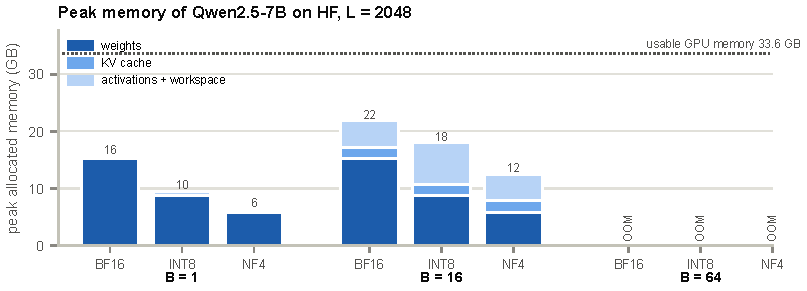
\includegraphics[width=\linewidth]{q1_memory_breakdown}
\caption{Peak allocated memory of Qwen2.5-7B on HF with 2048-token prompts, split into weights, KV
cache and activations. OOM: out of memory.}
\label{fig:breakdown}
\end{figure}

\begin{figure}[htbp]
\centering
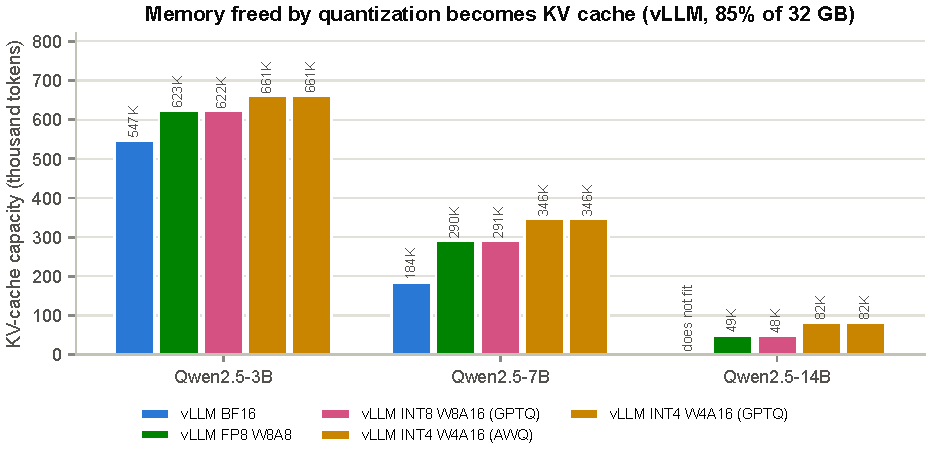
\includegraphics[width=\linewidth]{q1_kv_capacity}
\caption{KV-cache capacity that vLLM allocates with 85\% of the GPU after loading the weights.}
\label{fig:kvcap}
\end{figure}

\FloatBarrier
\section{Additional speed results}
\label{app:speed}

\Cref{tab:speed} lists the latency, throughput and energy numbers behind \cref{fig:latency}, and
\cref{tab:crossover} lists where each format stops paying off (\cref{fig:heatmaps}).
\Cref{fig:energy} shows the energy per output token. GPU power stays close to the board limit in
every configuration (\PowerRange\,W), so energy per token follows latency. LLM.int8() draws little
power (\PowerInt\,W) but runs so long that it uses the most energy per token. \Cref{fig:outlen}
shows how the answer length moves the speedup (\cref{sec:q3}).

\begin{table}[htbp]
\centering
\footnotesize
\caption{Latency, throughput and energy of Qwen2.5-7B with 512-token prompts and 128 output tokens (mean of 3 runs). Subscripts give the batch size. TTFT and TPOT in ms; Speedup$_1$ is the decode speedup over BF16 on the same backend; energy is GPU energy per output token.}
\label{tab:speed}
\setlength{\tabcolsep}{4pt}
\begin{tabular}{lrrrrrrr}
\toprule
Config & TTFT$_{1}$ & TPOT$_{1}$ & TPOT$_{64}$ & tok/s$_{64}$ & Speedup$_{1}$ & mJ/tok$_{1}$ & mJ/tok$_{64}$ \\
\midrule
HF BF16 & 38.4 & 10.90 & 20.04 & 1669 & 1.00$\times$ & 5092 & 294 \\
HF INT8 (LLM.int8) & 57.8 & 37.45 & 47.14 & 1003 & 0.29$\times$ & 6187 & 305 \\
HF NF4 & 48.3 & 9.62 & 22.87 & 1550 & 1.13$\times$ & 3188 & 340 \\
vLLM BF16 & 37.0 & 9.52 & 12.39 & 2209 & 1.00$\times$ & 4878 & 249 \\
vLLM FP8 W8A8 & 22.8 & 5.99 & 7.88 & 3886 & 1.59$\times$ & 2507 & 141 \\
vLLM GPTQ W8A16 & 38.5 & 5.80 & 8.41 & 2471 & 1.64$\times$ & 2588 & 234 \\
vLLM AWQ W4A16 & 38.6 & 3.90 & 7.99 & 2544 & 2.44$\times$ & 1919 & 224 \\
vLLM GPTQ W4A16 & 36.9 & 3.88 & 7.89 & 2642 & 2.45$\times$ & 1840 & 219 \\
\bottomrule
\end{tabular}
\end{table}

\begin{table}[htbp]
\centering
\footnotesize
\caption{Where each format stops paying off (Qwen2.5-7B, 512-token prompts, 128 output tokens). Speedup over BF16 on the same backend at batch size 1 and at the largest batch we ran (in brackets), and the batch size up to which the format is faster (linear interpolation in $\log B$).}
\label{tab:crossover}
\setlength{\tabcolsep}{3.5pt}
\begin{tabular}{lrrlrrl}
\toprule
 & \multicolumn{3}{c}{Decode step (TPOT)} & \multicolumn{3}{c}{Whole request (E2E)} \\
\cmidrule(lr){2-4}\cmidrule(lr){5-7}
Config & $B{=}1$ & largest $B$ & faster up to & $B{=}1$ & largest $B$ & faster up to \\
\midrule
HF INT8 (LLM.int8) & 0.29$\times$ & 0.43$\times$ (64) & never & 0.30$\times$ & 0.60$\times$ (64) & never \\
HF NF4 & 1.13$\times$ & 0.88$\times$ (64) & $B\approx7$ & 1.12$\times$ & 0.93$\times$ (64) & $B\approx7$ \\
vLLM FP8 W8A8 & 1.59$\times$ & 1.36$\times$ (256) & all $B$ & 1.59$\times$ & 1.73$\times$ (256) & all $B$ \\
vLLM GPTQ W8A16 & 1.64$\times$ & 1.00$\times$ (256) & $B\approx251$ & 1.61$\times$ & 0.97$\times$ (256) & $B\approx123$ \\
vLLM AWQ W4A16 & 2.44$\times$ & 1.02$\times$ (256) & all $B$ & 2.33$\times$ & 0.98$\times$ (256) & $B\approx175$ \\
vLLM GPTQ W4A16 & 2.45$\times$ & 1.05$\times$ (256) & all $B$ & 2.35$\times$ & 1.03$\times$ (256) & all $B$ \\
\bottomrule
\end{tabular}
\end{table}


\begin{figure}[htbp]
\centering
\begin{minipage}[t]{0.46\linewidth}
\centering
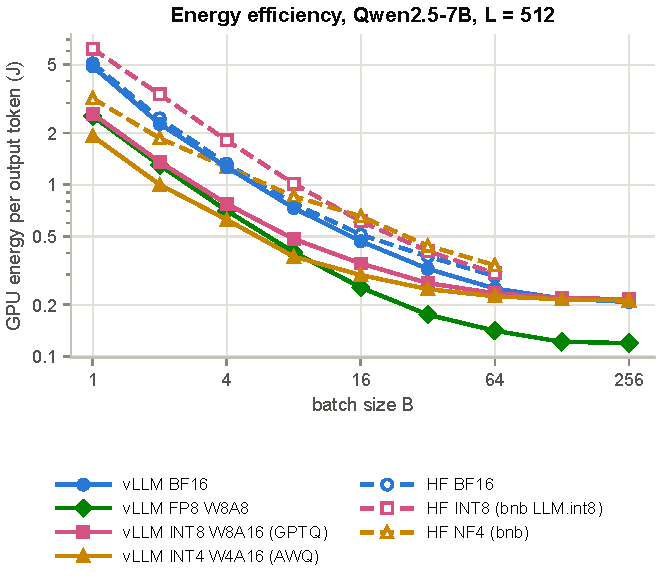
\includegraphics[width=\linewidth]{energy_per_token}
\caption{GPU energy per output token (NVML), Qwen2.5-7B, 512-token prompts.}
\label{fig:energy}
\end{minipage}\hfill
\begin{minipage}[t]{0.5\linewidth}
\centering
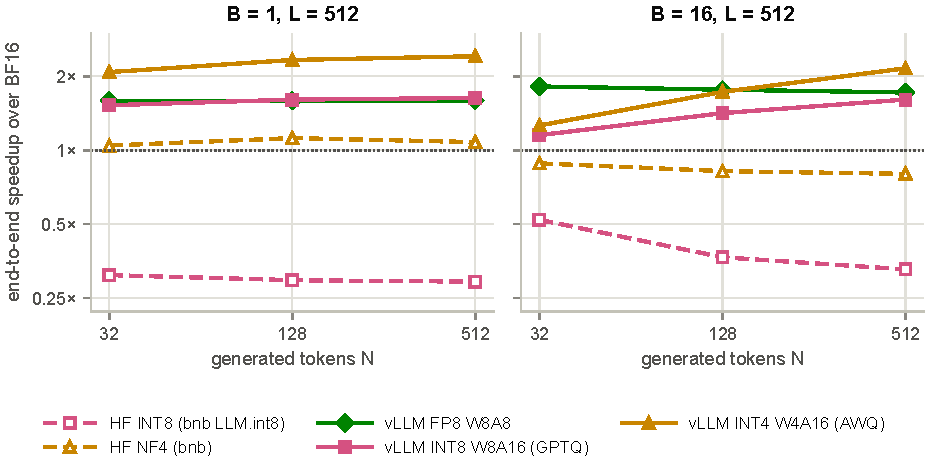
\includegraphics[width=\linewidth]{q3_output_length}
\caption{End-to-end speedup over BF16 against the number of generated tokens (Qwen2.5-7B, 512-token
prompts). Longer answers raise the share of decode, and with it the gain of weight-only formats.}
\label{fig:outlen}
\end{minipage}
\end{figure}

\textbf{Qwen2.5-3B.} \Cref{fig:latency3b,fig:heatmaps3b} repeat the latency and crossover analysis
for the 3B model. On vLLM the picture is the same as for 7B. On HF the smaller model is worse off. Its
BF16 step is already limited by the host (\TPOTbfHFThree\,ms per step against a memory floor of
\FloorThree\,ms), so fewer bytes cannot help: NF4 never beats BF16, and LLM.int8() falls to
\IntThreeWorst{} of the BF16 speed, because the 36-layer model launches more kernels per step than
the 28-layer 7B model.

\begin{figure}[htbp]
\centering
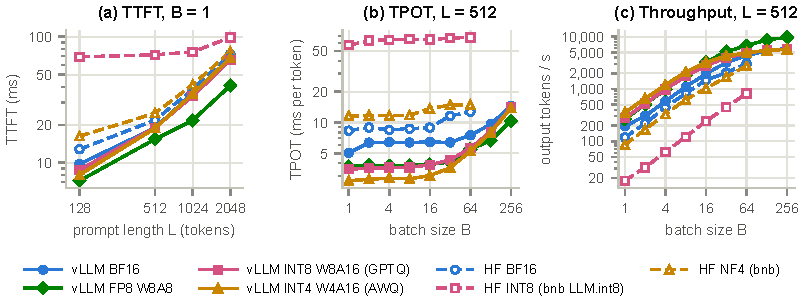
\includegraphics[width=\linewidth]{q2_latency_throughput_3b}
\caption{Latency and throughput of Qwen2.5-3B (same layout as \cref{fig:latency}).}
\label{fig:latency3b}
\end{figure}

\begin{figure}[htbp]
\centering
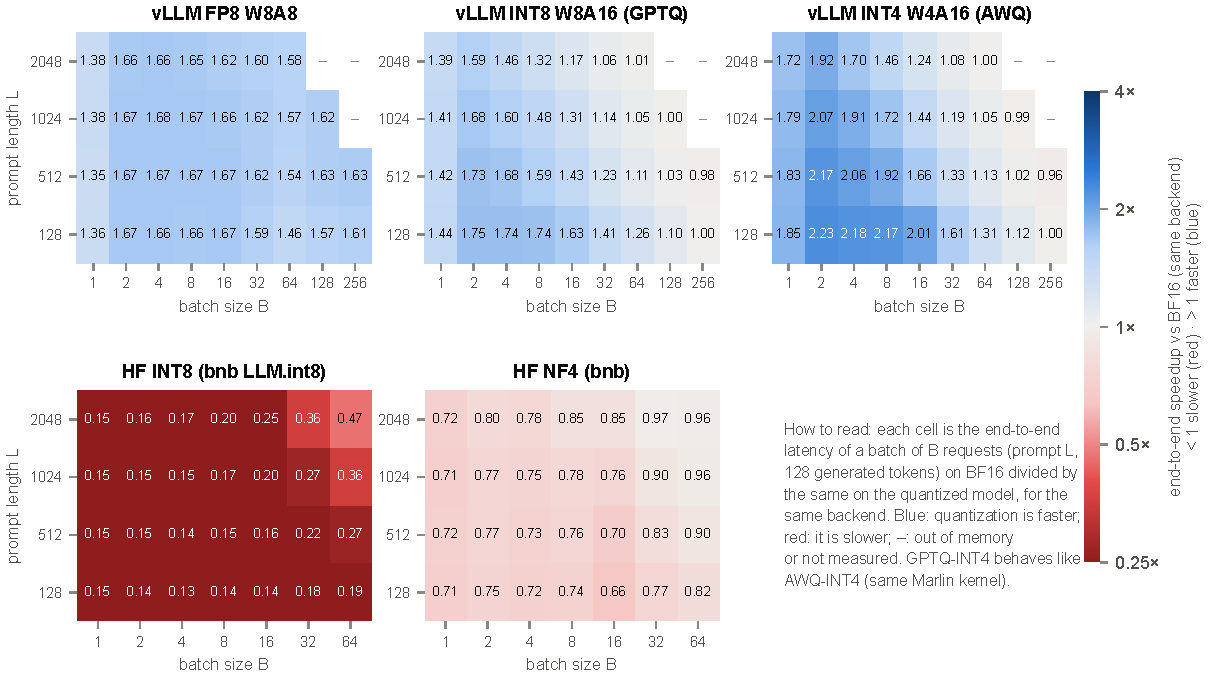
\includegraphics[width=\linewidth]{q3_speedup_heatmaps_3b}
\caption{End-to-end speedup over BF16 for Qwen2.5-3B (same layout as \cref{fig:heatmaps}).}
\label{fig:heatmaps3b}
\end{figure}

\FloatBarrier
\section{Real-traffic details}
\label{app:real}

\Cref{tab:serving_main} summarizes the ShareGPT replay of \cref{sec:real}. \Cref{fig:workload} shows
the lengths of the 300 requests, and \cref{fig:serving,tab:serving} give the full serving results,
including the 99th-percentile latencies.

\begin{table}[htbp]
\centering
\small
\caption{Real traffic: 300 ShareGPT requests replayed against Qwen2.5-7B with their reference answer lengths. $C$ is the number of concurrent requests (HF runs static batches of 16). Output tokens per second, and median TTFT and TPOT in ms.}
\label{tab:serving_main}
\setlength{\tabcolsep}{5pt}
\begin{tabular}{lrrrrrr}
\toprule
 & \multicolumn{2}{c}{$C=1$} & \multicolumn{2}{c}{$C=16$} & \multicolumn{2}{c}{$C=64$} \\
\cmidrule(lr){2-3}\cmidrule(lr){4-5}\cmidrule(lr){6-7}
Config & tok/s & TPOT & tok/s & TTFT & tok/s & TPOT \\
\midrule
HF BF16 (static) & -- & -- & 254 & 797 & -- & -- \\
HF INT8 (static) & -- & -- & 119 & 691 & -- & -- \\
HF NF4 (static) & -- & -- & 215 & 842 & -- & -- \\
\midrule
vLLM BF16 & 104 & 9.6 & 1,334 & 34 & 3,537 & 13.6 \\
vLLM FP8 & 164 & 6.1 & 2,237 & 21 & 5,388 & 8.9 \\
vLLM GPTQ-8 & 166 & 6.0 & 2,166 & 22 & 4,733 & 10.5 \\
vLLM AWQ-4 & 240 & 4.1 & 3,020 & 18 & 5,180 & 10.1 \\
vLLM GPTQ-4 & 241 & 4.1 & 2,970 & 18 & 5,181 & 10.0 \\
\bottomrule
\end{tabular}
\end{table}


\begin{figure}[htbp]
\centering
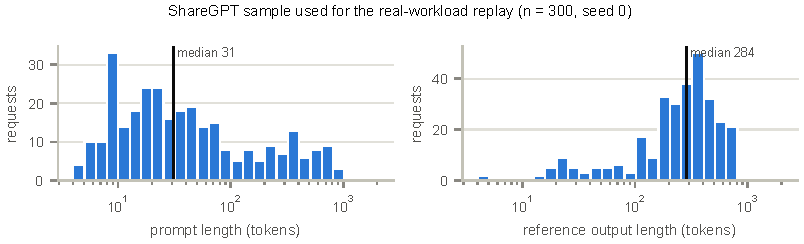
\includegraphics[width=\linewidth]{workload_sharegpt}
\caption{Prompt and answer lengths of the 300 ShareGPT requests used in the replay.}
\label{fig:workload}
\end{figure}

\begin{figure}[htbp]
\centering
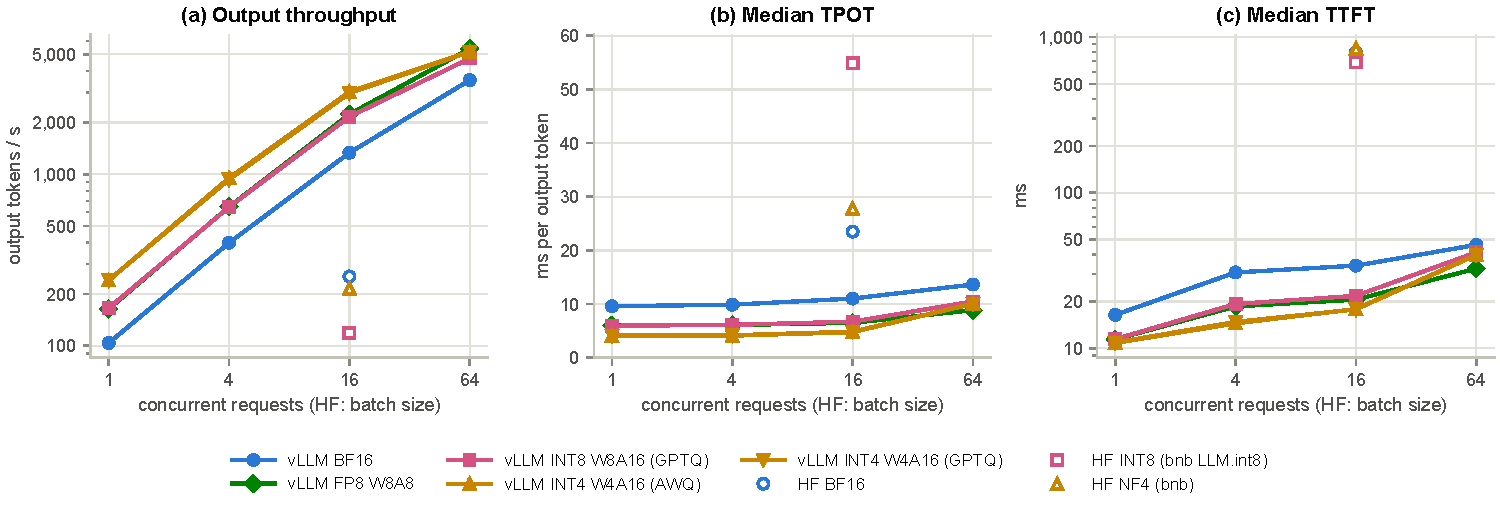
\includegraphics[width=\linewidth]{real_sharegpt_serving}
\caption{The ShareGPT replay against Qwen2.5-7B: vLLM at 1 to 64 concurrent clients (lines) and HF
with static batches of 16 (hollow markers). TTFT and TPOT are medians over requests.}
\label{fig:serving}
\end{figure}

\begin{table}[t]
\centering
\footnotesize
\caption{Real workload --- 300 ShareGPT requests replayed against Qwen2.5-7B (reference output lengths). $C$: concurrent closed-loop clients for vLLM, static batch size for HF. Throughput in requests/s and output tokens/s; TTFT and TPOT in ms.}
\label{tab:serving}
\setlength{\tabcolsep}{3.2pt}
\begin{tabular}{lrrrrr}
\toprule
Config & $C$ & req/s & tok/s & TTFT p50 / p99 & TPOT p50 / p99 \\
\midrule
vLLM BF16 & 1 & 0.35 & 104 & 16 / 62 & 9.6 / 9.6 \\
vLLM BF16 & 64 & 11.76 & 3537 & 46 / 1654 & 13.6 / 16.7 \\
vLLM FP8 & 1 & 0.54 & 164 & 11 / 44 & 6.1 / 6.2 \\
vLLM FP8 & 64 & 17.92 & 5388 & 33 / 1485 & 8.9 / 15.1 \\
vLLM GPTQ-8 & 1 & 0.55 & 166 & 11 / 63 & 6.0 / 6.2 \\
vLLM GPTQ-8 & 64 & 15.74 & 4733 & 41 / 1743 & 10.5 / 18.0 \\
vLLM AWQ-4 & 1 & 0.80 & 240 & 11 / 65 & 4.1 / 4.5 \\
vLLM AWQ-4 & 64 & 17.23 & 5180 & 40 / 1747 & 10.1 / 14.8 \\
vLLM GPTQ-4 & 1 & 0.80 & 241 & 11 / 62 & 4.1 / 4.4 \\
vLLM GPTQ-4 & 64 & 17.23 & 5181 & 40 / 1722 & 10.0 / 19.3 \\
\bottomrule
\end{tabular}
\end{table}


\FloatBarrier
\section{Full quality results}
\label{app:quality}

\Cref{tab:quality} lists every quality number with its $p$-value, for all five models.

\begin{table}[t]
\centering
\footnotesize
\caption{Q4 --- quality. WikiText-2 perplexity (2048-token windows) and GSM8K accuracy (1,319 questions, zero-shot CoT, greedy decoding). Deltas are against HF BF16 of the same model; $p$ is the two-sided exact McNemar test of the paired GSM8K answers against HF BF16.}
\label{tab:quality}
\setlength{\tabcolsep}{3.2pt}
\begin{tabular}{llrrrrr}
\toprule
Model & Config & PPL & $\Delta$PPL & GSM8K (\%) & $\Delta$acc & $p$ \\
\midrule
3B & HF BF16 & 8.56 & -- & 85.8 & -- & -- \\
 & HF INT8 & 8.66 & $+0.10$ & 85.5 & $-0.3$ & 0.777 \\
 & HF NF4 & 9.11 & $+0.55$ & 82.6 & $-3.3$ & $<$0.001 \\
 & vLLM BF16 & 8.56 & $+0.00$ & 86.0 & $+0.2$ & 0.871 \\
 & vLLM FP8 & 8.64 & $+0.09$ & 85.4 & $-0.5$ & 0.610 \\
 & vLLM GPTQ-8 & 8.56 & $+0.00$ & 86.4 & $+0.6$ & 0.322 \\
 & vLLM AWQ-4 & 9.10 & $+0.54$ & 82.7 & $-3.1$ & 0.002 \\
 & vLLM GPTQ-4 & 9.22 & $+0.66$ & 82.0 & $-3.8$ & $<$0.001 \\
7B & HF BF16 & 7.46 & -- & 90.8 & -- & -- \\
 & HF INT8 & 7.49 & $+0.03$ & -- & -- & -- \\
 & HF NF4 & 7.77 & $+0.31$ & 90.3 & $-0.5$ & 0.500 \\
 & vLLM BF16 & 7.46 & $+0.00$ & 91.2 & $+0.4$ & 0.359 \\
 & vLLM FP8 & 7.51 & $+0.05$ & 90.8 & $+0.0$ & 1.000 \\
 & vLLM GPTQ-8 & 7.46 & $+0.00$ & 91.7 & $+0.9$ & 0.043 \\
 & vLLM AWQ-4 & 7.85 & $+0.39$ & 90.4 & $-0.5$ & 0.576 \\
 & vLLM GPTQ-4 & 7.78 & $+0.32$ & 91.1 & $+0.2$ & 0.828 \\
14B & vLLM FP8 & 5.77 & -- & 94.4 & -- & -- \\
 & vLLM GPTQ-8 & 5.71 & -- & 94.7 & -- & -- \\
 & vLLM AWQ-4 & 6.16 & -- & 93.9 & -- & -- \\
 & vLLM GPTQ-4 & 37.46$^{\ddagger}$ & -- & 93.7 & -- & -- \\
\bottomrule
\end{tabular}
\par\vspace{2pt}\parbox{\linewidth}{\scriptsize $^{\ddagger}$Degraded on raw text but not on chat-formatted text; see \cref{sec:q4}.}
\end{table}


\FloatBarrier
\section{Generalization details}
\label{app:general}

\Cref{tab:general} compares Qwen2.5-7B and Qwen3-8B on the same grid.

\begin{table}[htbp]
\centering
\small
\caption{The main results for Qwen2.5-7B and Qwen3-8B (non-thinking mode) on the same grid (512-token prompts, 128 output tokens). Throughput is compared at the largest batch at which both models' KV caches hold every request ($B=64$). Qwen3-8B has no official GPTQ checkpoint.}
\label{tab:general}
\setlength{\tabcolsep}{3.2pt}
\begin{tabular}{lrr}
\toprule
Metric (vs.\ BF16) & Qwen2.5-7B & Qwen3-8B \\
\midrule
Weight saving, AWQ-INT4 (vLLM) & 2.70$\times$ & 2.67$\times$ \\
Weight saving, NF4 (HF) & 2.60$\times$ & 2.55$\times$ \\
Decode speedup $B=1$, AWQ-INT4 & 2.44$\times$ & 2.33$\times$ \\
Decode speedup $B=1$, FP8 & 1.59$\times$ & 1.54$\times$ \\
Decode speedup $B=1$, NF4 & 1.13$\times$ & 0.90$\times$ \\
Decode speedup $B=1$, LLM.int8() & 0.29$\times$ & 0.28$\times$ \\
Throughput $B=64$, AWQ-INT4 & 1.15$\times$ & 1.12$\times$ \\
Throughput $B=64$, FP8 & 1.76$\times$ & 1.67$\times$ \\
GSM8K $\Delta$ pp ($p$), FP8 & $0.0$ (1.000) & $+0.5$ (0.488) \\
GSM8K $\Delta$ pp ($p$), LLM.int8() & $-0.2$ (0.771) & $+0.6$ (0.382) \\
GSM8K $\Delta$ pp ($p$), AWQ-INT4 & $-0.5$ (0.576) & $-0.2$ (0.818) \\
GSM8K $\Delta$ pp ($p$), NF4 & $-0.5$ (0.500) & $+0.2$ (0.909) \\
MMLU $\Delta$ pp ($p$), FP8 & $-0.1$ (0.327) & $-0.7$ ($<$0.001) \\
MMLU $\Delta$ pp ($p$), LLM.int8() & $-0.2$ (0.134) & $+0.7$ ($<$0.001) \\
MMLU $\Delta$ pp ($p$), AWQ-INT4 & $-1.6$ ($<$0.001) & $-0.7$ (0.003) \\
MMLU $\Delta$ pp ($p$), NF4 & $-0.6$ (0.002) & $-0.3$ (0.156) \\
\bottomrule
\end{tabular}
\end{table}


\FloatBarrier
\section{Reproducibility}
\label{app:repro}
Every number in this report is computed from the raw measurements by \texttt{scripts/make\_numbers.py},
and the figures and tables come from \texttt{make\_figures.py} and \texttt{make\_tables.py}.
\texttt{run\_all.sh} runs all experiments again (about twelve GPU-hours on an RTX 5090). A job queue
ran the experiments one at a time, and only while no other user's process was on the GPU. Rows
written while the GPU was shared (\ExcludedWindows, logged in \texttt{results/excluded\_windows.jsonl})
were discarded and those jobs were run again. \RecheckSentence
